
% Manual de Marca do Núcleo de Estudos e Pesquisas Experimentais e Tecnológicas (NExT)
% Utilizar o xelatex para compilar
% Autor: Pedro Maione [pedromaione@gmail.com]

\documentclass{manualmarca}

% \usepackage{showframe}

\TituloDocumento{Manual de Identidade Visual}
\AutorDocumento{Pedro Maione}
\DataDocumento{03/05/2017}
\VersaoDocumento{2017v01}

\graphicspath{%
  {./../fig/},
  {./../eps/},
}

\begin{document}

\maketitle{}

% \tableofcontents{}

\InicioDocumento{}

\chapter{Código de identidade visual}
\label{cha:codigo-de-identidade}

\section{Características Gerais}
\label{sec:caract-gerais}

O logotipo do \NExT{}  é composto pelas letras que representão a sigla no Núcleo.

\vspace*{1cm}
\begin{figure}[!htp]
  \centering
  
\includegraphics[scale=1]{logo-next-color}
\end{figure}
\vspace*{\stretch{1}}

\noindent Outra opção do logotipo é a composta por símbolo e texto.

\vspace*{1cm}
\begin{figure}[!htp]
  \centering
  
\includegraphics[scale=1]{logo-next-inline}
\end{figure}
\vspace*{1cm}
\begin{figure}[!htp]
  \centering
  
\includegraphics[scale=1]{logo-next-stacked}
\end{figure}
\vspace*{\stretch{1}}

\noindent
Existe ainda a opção do logotipo com efeito de sombra, ilustrado abaixo.

\vspace*{1cm}
\begin{figure}[!htp]
  \centering
  
\includegraphics[scale=1]{logo-next-shade}
\end{figure}
\vspace*{\stretch{1}}

\pagebreak[4]

\section{Área de não-interferência}
\label{sec:area-de-nao}

\begin{figure}[!htp]
  \centering
  \begin{minipage}{.32\textwidth}
    Para assegurar a correta percepção, caso associado a outros elementos visuais, é necessário deixar uma área livre em volta do logotipo, conforme o diagrama ao lado.

    Sendo que o mesmo vale para o logotipo com símbolo e texto, conforme diagrama abaixo.
  \end{minipage}%
  \hfill
  \begin{minipage}{.65\textwidth}
  \centering
  
\includegraphics[scale=1]{logo-next-clearspace}
\end{minipage}
\end{figure}

\vspace*{\stretch{1}}
\begin{figure}[!htp]
  \centering
  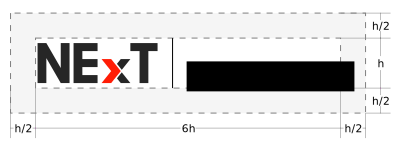
\includegraphics[scale=1]{logo-next-inline-clearspace}
\end{figure}

\vspace*{\stretch{1}}

\begin{figure}[!htp]
  \centering
  
\includegraphics[scale=1]{logo-next-stacked-clearspace}
\end{figure}
\vspace*{\stretch{1}}
\pagebreak[4]

\section{Construção do logotipo}
\label{sec:const-logotipo}

\begin{figure}[!htp]
  \centering
  \begin{minipage}{.32\textwidth}
    As linhas na cor {\color[named]{magenta} magenta} indicam as proporções verticais. A altura do logotipo (\emph{$H$}) é subdividida em 5 (cinco) partes, denotando a unidade $x$, que é a base para definir as linhas de grade.
    
    As linhas na cor {\color{black!30!green} verde} indicam as proporções horizontais do logotipo. A largura total (\emph{L}) do logotipo é de 3 (três) vezes a altura (\emph{H}).

    As linhas na cor {\color{orange} laranja} representam o \emph{offset} da seta da letra ``x'' do logotipo.
  \end{minipage}%
  \hfill
  \begin{minipage}{.65\textwidth}
  \centering
  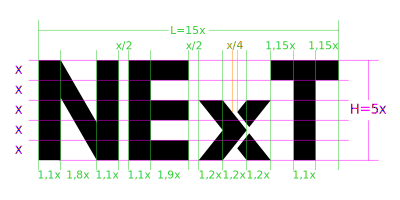
\includegraphics[scale=1]{logo-next-grid}
\end{minipage}
\end{figure}

\vspace*{\stretch{1}}

\noindent Os logotipos com símbolo e texto foram construidos como indicam os diagramas abaixo.

\begin{figure}[!htp]
  \centering
  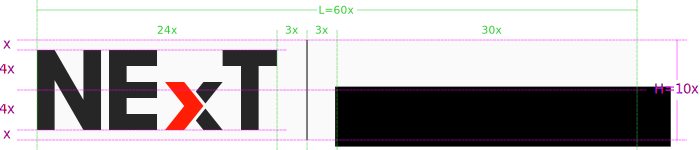
\includegraphics[width=\textwidth]{logo-next-inline-grid}
\end{figure}

\vspace*{\stretch{1}}

\begin{figure}[!htp]
  \centering
  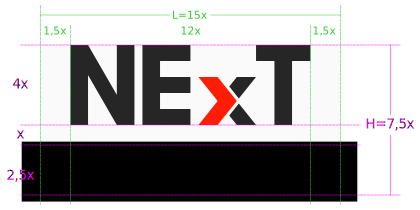
\includegraphics[scale=1]{logo-next-stacked-grid}
\end{figure}

\vspace*{\stretch{1}}

\pagebreak[4]

\section{Fontes}
\label{sec:fontes-padrao}

A fonte utilizado para o logotipo foi a \emph{League Spartan}, obtida no \href{https://www.fontsquirrel.com/fonts/league-spartan}{Font Squirrel}, e está definida sob a licensa \emph{SIL Open Font License v1.10}. No entanto, foi necessário adequar ao grid, gerando uma variação em relação à fonte original.

\vspace*{1cm}

\begin{figure}[!htp]
  \centering
  
\includegraphics[width=.8\textwidth]{league-spartan_720x300.png}
\end{figure}

\vspace*{\stretch{1}}

\begin{figure}[!htp]
  \centering
  \begin{minipage}[l]{.32\textwidth}
    Para ilustrar as alterações realizadas em relação à fonte original temos a imagem ao lado.
  \end{minipage}%
  \hfill%
  \begin{minipage}[r]{.6\textwidth}
    \centering
    
\includegraphics[scale=1]{logo-next-comparacao}
  \end{minipage}
\end{figure}

\vspace*{\stretch{1}}

\noindent Para os logotipos com símbolo e texto, é utilizado a fonte \emph{Roboto}, disponível no \href{https://fonts.google.com/specimen/Roboto}{Google~Fonts}.

\vspace*{1cm}
\begin{figure}[!htp]
  \centering
  
\includegraphics[width=.8\textwidth]{roboto-720x300.png}
\end{figure}

\vspace*{\stretch{1}}

\pagebreak[4]

\section{Padrões Cromáticos}
\label{sec:padroes-cromaticos}

\subsection{Cores Primárias}
\label{sec:cores-primarias}

O símbolo do \NExT{} é composto por duas cores principais.

\vspace*{1cm}
\noindent
\begin{center}
  \DescricaoCor{FF1D06}{255, 29, 6}{0, 89, 98, 0}
  \DescricaoCor{262626}{38, 38, 38}{0, 0, 0, 85}
\end{center}
\vspace*{\stretch{1}}

\subsection{Cores Secundárias}
\label{sec:cores-secundarias}

\vspace*{1cm}
\noindent
\DescricaoCor{FF9206}{255, 146, 6}{0, 43, 98, 0}
\DescricaoCor{0E65A3}{14, 101, 163}{91, 38, 0, 36}
\DescricaoCor{04C02E}{4, 192, 46}{98, 0, 76, 25}
\vspace*{\stretch{1}}

\subsection{Variações}
\label{sec:variacoes}

Para obter uma paleta de cores com as variações, utilize os links abaixo:

\begin{itemize}
\item \href{http://paletton.com/#uid=7040D0kvjvXojH8rfABuGpcuRk9}{Paleta de cores}
\item \href{http://paletton.com/#uid=1000D0k004M0dcY0dcY5o003H00}{Paleta de escala de cinza}
\end{itemize}

\noindent
Para obtenção das paletas de cores, foi utilizado a ferramenta \href{http://paletton.com}{http://paletton.com}.

\vspace*{1cm}
\begin{figure}[!htp]
  \centering
  {Paleta de cores completa.}
  
\includegraphics[scale=1]{paleta-cores-escala}
\end{figure}

\vspace*{\stretch{1}}

\pagebreak[4]

\section{Escala de Redução}
\label{sec:escala-de-reducao}

O logotipo nunca deve ser reduzido a um tamanho menor que os indicados abaixo. Em cada diagrama está representado as dimensoẽs mínimas para apicações eletrônicas em \emph{pixels} e para impressão e publicação em \emph{milimetros}

\noindent
{\bfseries Atenção: Os valores entre parênteses, na cor {\color{magenta} magenta} não representam a conversão de \emph{pixels} para milimetros.}

\vspace*{\stretch{2}}

\begin{figure}[!htp]
  \centering
  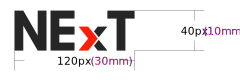
\includegraphics[scale=1]{logo-next-minimo}
\end{figure}
\vspace*{\stretch{1}}
\begin{figure}[!htp]
  \centering
  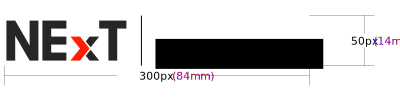
\includegraphics[scale=1]{logo-next-inline-minimo}
\end{figure}
\vspace*{\stretch{1}}
\begin{figure}[!htp]
  \centering
  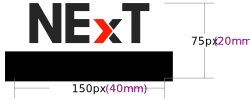
\includegraphics[scale=1]{logo-next-stacked-minimo}
\end{figure}

\vspace*{\stretch{2}}

\pagebreak[4]

\section{Variantes do Logotipo}
\label{sec:vari-do-logot}

As variações admitidas para o logotipo do \NExT{} estão reçacionadas abaixo, sendo:

\subsection{Versões colorida, positivo e negativo}

\begin{figure}[!htp]
  \centering
  
\includegraphics[scale=2]{logo-next-color-variacoes-01}
\end{figure}

\subsection{Versões monocromáticas, positivo e negativo}

\begin{figure}[!htp]
  \centering
  
\includegraphics[scale=2]{logo-next-color-variacoes-02}
\end{figure}

\subsection{Versões coloridas com sombra, positivo e negativo}

\begin{figure}[!htp]
  \centering
  
\includegraphics[scale=2]{logo-next-color-variacoes-03}
\end{figure}

\subsection{Outras variações do logotipo}

Podem ser obtidos outras variantes do logotipo, com a utilização dos logotipos com símbolo e texto, em linha ou empilhado, seguindo as orientações acima. Por exemplo:

\begin{figure}[!htp]
  \centering
  
\includegraphics[scale=1]{logo-next-color-variacoes-04}
\end{figure}

\vspace*{\stretch{1}}

\pagebreak[4]


% \chapter{Papelaria Institucional}
% \label{cha:papel-inst}

% \section{Papel de Carta}
% \label{sec:papel-de-carta}

% \section{Cartão de Visita}
% \label{sec:cartao-de-visita}

% \section{Envelope}
% \label{sec:envelope}

% \section{Modelo de Certificado}
% \label{sec:modelo-de-cert}

% \chapter{Padronização de publicações}
% \label{cha:padr-de-publ}

% \section{Projeto de Tipografia}
% \label{sec:proj-de-tipogr}

% \chapter{Assinatura de Logotipos}
% \label{cha:assin-de-logot}

\end{document}


%%% Local Variables: 
%%% coding: utf-8
%%% mode: latex
%%% TeX-engine: xetex
%%% TeX-master: t
%%% End: 
